\section*{Theorems}

% lecture 1
\begin{theorem}[L1.1]{Weierstrass.}
    Let $f: \Omega \rightarrow \mathbb{R}$ be a continuous function defined on a nonempty and compact (i.e., closed and bounded) set $\Omega$. Then, there exists a minimizer $x^* \in \Omega$ of $f$ on $\Omega$, that is,
    $$
    f\left(x^*\right) \leq f(x) \quad \text { for all } x \in \Omega
    $$
    \vspace{-5pt}
\end{theorem}

\begin{theorem}[L1.2]{Weierstrass for Compact Sublevel Sets.}
    Let $f$ be a continuous function defined on a set $S$. If $f$ has a nonempty and compact sublevel set, that is, there exists $\alpha \in \mathbb{R}$ such that
    $$
    \{x \in S: f(x) \leq \alpha\}
    $$
    is nonempty, bounded, and closed, then $f$ has a minimizing point in $S$.
\end{theorem}


% lecture 2

\begin{definition}[L2.1]{Star-convexity at $x$.} 
    A set $\Omega \subseteq \mathbb{R}^n$ is said to be star-convex at a point $x \in \Omega$ if, for all $y \in \Omega$, the entire segment from $x$ to $y$ is contained in $\Omega$. In symbols, if
    \vspace{-5pt}\\
    $$
    x+t \cdot(y-x) \in \Omega \quad \forall t \in[0,1]
    $$
    \vspace{-10pt}\\
    (Note that the condition is equivalent to \\
    "$t \cdot y+(1-t) \cdot x \in \Omega$ $\forall$ $y \in \Omega$, $t \in$ $[0,1]$ ", or also \\
    "$t \cdot x+(1-t) \cdot y \in \Omega$ $\forall$ $y \in \Omega$, $t \in[0,1]$ ".)
\end{definition}

\begin{definition}[L2.2]{Convex set.} 
    A set $\Omega$ is convex if it is star-convex at all of its points $x \in$ $\Omega$. In other words, $\Omega$ is convex if all segments formed between any two points $x, y \in \Omega$ are entirely contained in $\Omega$. In symbols, if
    \vspace{-5pt}\\
    $$
    t \cdot x+(1-t) \cdot y \in \Omega \quad \forall x, y \in \Omega \text { and } t \in[0,1] .
    $$
    \vspace{-5pt}
\end{definition}

\begin{theorem}[L2.1]{First-order necessary condition for a convex feasible set}
    Let $\Omega \subseteq \mathbb{R}^n$ be convex and $f: \mathbb{R}^n \rightarrow \mathbb{R}$ be a differentiable function. For a point $x \in \Omega$ to be a minimizer of $f$ over $\Omega$ it is necessary that
    \vspace{-5pt}\\
    $$
    \langle\nabla f(x), y-x\rangle \geq 0 \quad \forall y \in \Omega
    $$
    \vspace{-5pt}
\end{theorem}

\begin{definition}[L2.3]{Normal cone.}
    Let $\Omega \subseteq \mathbb{R}^n$ be convex, and let $x \in \Omega$. The normal cone to $\Omega$ at $x$, denoted $\mathcal{N}_{\Omega}(x)$, is defined as the set
    \vspace{-5pt}\\
    $$
    \mathcal{N}_{\Omega}(x):=\left\{d \in \mathbb{R}^n:\langle d, y-x\rangle \leq 0 \quad \forall y \in \Omega\right\} .
    $$
    \vspace{-5pt}\\
    With this definition, the first-order necessary optimality condition for $x$, given in Th L2.1, can be equivalently written as
    \vspace{-5pt}\\
    $$
    -\nabla f(x) \in \mathcal{N}_{\Omega}(x)
    $$
    \vspace{-5pt}
\end{definition}

\begin{theorem}[L2.2]{Normal cone to a hyperplane.}
\begin{minipage}[c]{0.65\textwidth}
    Consider a hyperplane
    \vspace{-5pt}\\
    $$
    \Omega := \{y \in \mathbb{R}^n : \langle a, y \rangle = 0\},
    $$
    \vspace{-10pt}\\
    where $a \in \mathbb{R}^n,\, a \neq 0,$
    and a point $x \in \Omega$. The normal cone at $x$ is given by
    \vspace{-5pt}\\
    $$
    \mathcal{N}_{\Omega}(x) = \operatorname{span}\{a\} = \{\lambda a : \lambda \in \mathbb{R}\}.
    $$
\end{minipage}\hfill
\begin{minipage}[c]{0.32\textwidth}
    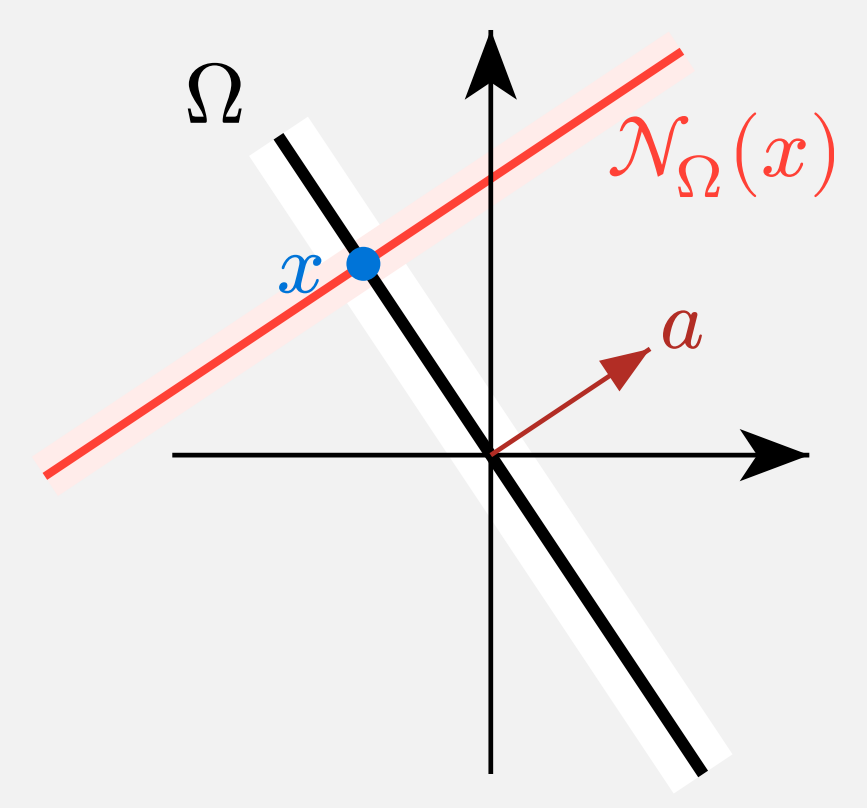
\includegraphics[width=\linewidth]{figures/normal_cone_hyperplane}
\end{minipage}
\end{theorem}

% lecture 3

\begin{theorem}[L3.1,L5.3]{Normal cone to the intersection of m halfspaces.}
    Let $\Omega \subseteq \mathbb{R}^n$ be given as the intersection of $m$ linear inequalities $\langle a_j, x\rangle \leq b_j$. Then, the normal cone at any point $x \in \Omega$ is obtained by taking nonnegative combinations of all those $a_j$ 's for which $\langle a_j, x\rangle=b_j$. 
    \vspace{-5pt}\\
    $$
    \mathcal{N}_{\Omega}(x)=\left\{\sum_{j \in I(x)} \lambda_j \cdot a_j: \lambda_j \in \mathbb{R}_{\geq 0}\right\},
    $$ 
    \vspace{-5pt}\\
    where $I(x)=\left\{j \in\{1, \ldots, m\}:\langle a_j, x\rangle=b_j\right\}$.\\
    The constraints $j$ in $I(x)$ are often called the "active constraints" at $x \in \Omega$.
    Alternatively in vectorial form let $Ax \leq b$, then with $A\in \mathbb{R}^{m \times n}, b \in \mathbb{R}^m$:
    \vspace{-5pt}\\
    $$
    \mathcal{N}_{\Omega}(x)=\left\{A^{\top} \lambda: \lambda^{\top}(b-A x)=0, \lambda \in \mathbb{R}_{\geq 0}^m\right\},
    $$
    \vspace{-10pt}\\
    $$
    A=\left(\begin{array}{c}
        -a_1^{\top}- \\
        \vdots \\
        -a_m^{\top}-
        \end{array}\right),
    $$
    rewriting the condition $j \in I(x)$ (via \textbf{complementary slackness}).
\end{theorem}

\begin{theorem}[L3.2]{Strong linear programming duality.}
    If (P) admits an optimal solution $x^*$, then (D) admits an optimal solution $\lambda^*$, such that:
    \begin{itemize}[leftmargin=*]
        \item the values of the two problems coincide: $c^{\top} x^*=b^{\top} \lambda^*$, and
        \item   $\lambda^*$ satisfies the complementary slackness condition $(\lambda^*)^{\top}(b-A x^*)=0$.
    \end{itemize} 
\end{theorem}

% lecture 4

\begin{definition}[L4.1]{Convex function.}\hfill
    \vspace{2pt}
    \begin{minipage}[c]{0.65\textwidth}
        Let $\Omega \subseteq \mathbb{R}^n$ be convex.
        A function $f: \Omega \rightarrow \mathbb{R}$ is convex if, for any two points $x, y \in \Omega$ and $t \in[0,1]$,
        \vspace{-5pt}\\
        $$
        f((1-t) \cdot x+t \cdot y) \leq
        $$
        \vspace{-10pt}
        $$
        \quad (1-t) \cdot f(x)+t \cdot f(y)
        $$
        \vspace{-5pt}
    \end{minipage}\hfill
    \begin{minipage}[c]{0.32\textwidth}
        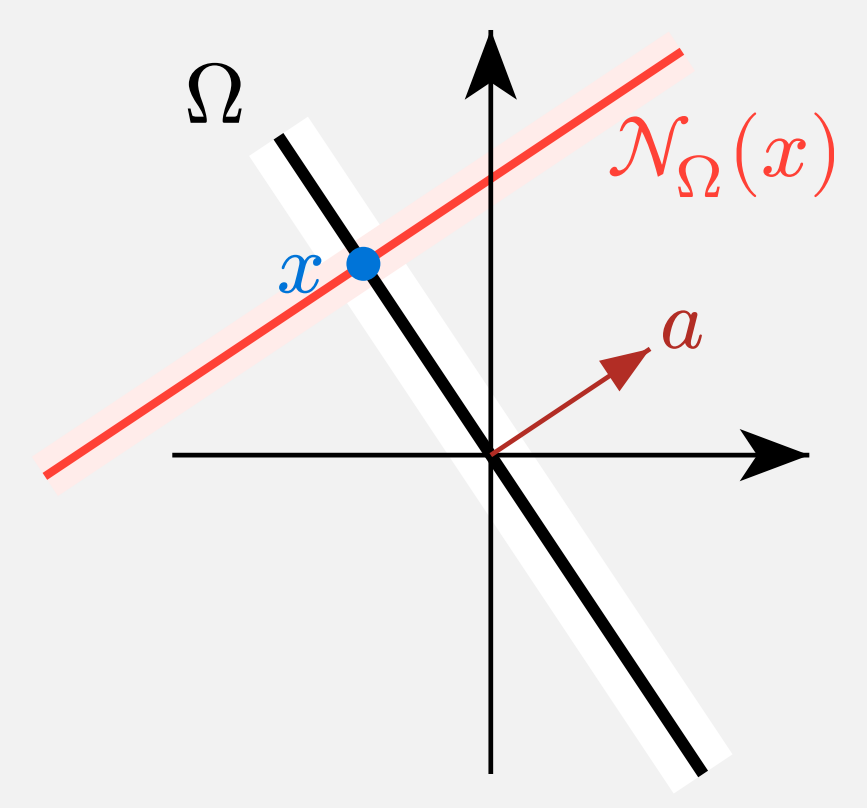
\includegraphics[width=\linewidth]{figures/normal_cone_hyperplane}
    \end{minipage}  
\end{definition}

\begin{theorem}[L4.1]{}
    Let $f: \Omega \rightarrow \mathbb{R}$ be a convex and differentiable function defined on a convex domain $\Omega$. Then, at all $x \in \Omega$,
    \vspace{-5pt}\\
    $$
    f(y) \geq \underbrace{f(x)+\langle\nabla f(x), y-x\rangle}_{\text {linearization of } f \text { around } x} \quad \forall y \in \Omega .
    $$
    \vspace{-5pt}
\end{theorem}

\begin{theorem}[L4.2]{Sufficiency of first-order optimality condition.}
    Let $\Omega \subseteq \mathbb{R}^n$ be convex and $f: \Omega \rightarrow \mathbb{R}$ be a convex differentiable function. Then,
    \vspace{-5pt}\\
    \begin{equation*}
        \begin{aligned}
            -\nabla f(x) \in \mathcal{N}_{\Omega}(x) \quad \Longleftrightarrow \quad & \text{$x$ is a minimizer of } \\
            & \text{$f$ on $\Omega$}
        \end{aligned}
    \end{equation*}
    \vspace{-5pt}
\end{theorem}

\begin{theorem}[L4.3]{Equivalent definitions of convexity.}
    Let $\Omega \subseteq \mathbb{R}^n$ be a convex set, and $f: \Omega \rightarrow \mathbb{R}$ be a function. The following are equivalent definitions of convexity for $f$ :
    \vspace{-5pt}
    \begin{enumerate}[leftmargin=*]
        \item $f((1-t) x+t y) \leq(1-t) f(x)+t f(y)$ for all $x, y \in \Omega, t \in[0,1]$.
        \item $f(y) \geq f(x)+\langle\nabla f(x), y-x\rangle$ for all $x, y \in \Omega$ [If $f$ is differentiable]
        \item $\langle\nabla f(y)-\nabla f(x), y-x\rangle \geq 0$ for all $x, y \in \Omega$ [If $f$ is differentiable]
        \item $\nabla^2 f(x) \succeq 0$ for all $x \in \Omega$ [If $f$ is twice differentiable and $\Omega$ is open]
    \end{enumerate}
    \vspace{-5pt}
\end{theorem}

\begin{theorem}[L4.4]{Operations preserving convexity.}
    \begin{itemize}[leftmargin=*]
        \item Multiplication of a convex function $f(x)$ by a nonnegative scalar $c \geq 0$;
        \item Addition of two convex functions $f(x), g(x)$;
        \item Pointwise supremum of a collection $J$ of convex functions $\left\{f_j(x): j \in J\right\}$ :
        \vspace{-5pt}\\
        $$
        f_{\max }(x):=\max _{j \in J} f_j(x) ;
        $$
        \vspace{-10pt}
        \item Pre-composition $f(A x+b)$ of a convex function $f$ with an affine function $A x+b$.
        \item Post-composition $g(f(x))$ of a convex function with an increasing convex function $g$;
        \item Infimal convolution $f \pm g$ of two convex functions $f, g: \mathbb{R}^n \rightarrow \mathbb{R}$, defined as
        \vspace{-5pt}\\
        $$
        \inf \left\{f(y)+g(x-y): y \in \mathbb{R}^n\right\}
        $$
        \vspace{-5pt}
    \end{itemize}

\end{theorem}

\begin{definition}[L4.2]{Strict and strong convexity.}
    Let $\Omega \subseteq \mathbb{R}^n$ be convex.
    \begin{itemize}[leftmargin=*]
        \item A function $f: \Omega \rightarrow \mathbb{R}$ is strictly convex if, for any two distinct points $x, y \in \Omega$ and $t \in(0,1)$,
        \vspace{-5pt}\\
        $$
        f((1-t) \cdot x+t \cdot y)<(1-t) \cdot f(x)+t \cdot f(y)
        $$
        \vspace{-10pt}
        \item A function $f: \Omega \rightarrow \mathbb{R}$ is strongly convex with modulus $\mu>0$ if the function
        \vspace{-5pt}\\
        $$
        f(x)-\frac{\mu}{2}\|x\|_2^2
        $$
        \vspace{-10pt}\\
        is convex.
        Note that strong convexity implies strict convexity, and strict convexity implies convexity. Neither of the reverse implications holds.
    \end{itemize}
\end{definition}

\begin{theorem}[L4.5]{Strict convexity and uniqueness of minimizer.}
    Let $\Omega \subseteq \mathbb{R}^n$ be convex, and $f: \Omega \rightarrow \mathbb{R}$ be a strictly convex function. Then, $f$ has at most one minimizer.\\
    \textbf{Corollary (Projection onto convex set):} Since the function $\|x-y\|_2^2$ is strongly convex, and hence strictly convex, it follows that any projection onto a convex set $\Omega$, if it exists, is unique. 
\end{theorem}

% lecture 5

\begin{theorem}[L5.1]{Separation}
    Let $\Omega \subseteq \mathbb{R}^n$ be a nonempty, closed, and convex set, and let $y \in \mathbb{R}^n$ be a point. If $y \notin \Omega$, then there exist $u \in \mathbb{R}^n, v \in \mathbb{R}$ such that
    \vspace{-5pt}\\
    $$
    \langle u, y\rangle<v, \quad \text { and } \quad\langle u, x\rangle \geq v \quad \forall x \in \Omega .
    $$
    \vspace{-5pt}\\
    \textbf{Note:} Also works for strict inequalities if we choose v so that the havspace passes through midpoint of line connecting y and $x^\star$.
\end{theorem}

\begin{definition}[L5.1]{Cone}
    A set $S$ is a cone if, for any $x \in S$ and $\lambda \in \mathbb{R}_{\geq 0}$, the point $\lambda \cdot x \in S$.
\end{definition}

\begin{theorem}[L5.2]{Separation of a point from a cone.}
    Let $S \subseteq \mathbb{R}^n$ be a nonempty closed convex cone, and $y \notin S$ be a point in $\mathbb{R}^n$. Then, there exists a hyperplane passing through the origin that separates $y$ from $S$; formally, there exists $u \in \mathbb{R}^n$ such that
    \vspace{-5pt}\\
    $$
    \langle u, y\rangle<0 \quad \text { and } \quad\langle u, x\rangle \geq 0 \quad \forall x \in S
    $$
    \vspace{-5pt}
\end{theorem}

\begin{definition}[L5.2]{(Strong) separation oracle}
    Let $\Omega \subseteq \mathbb{R}^n$ be convex and closed. A strong separation oracle for $\Omega$ is an algorithm that, given any point $y \in \mathbb{R}^n$, correctly outputs one of the following:
    \begin{itemize}[leftmargin=*]
        \item " $y \in \Omega$ ", or
        \item $(y \notin \Omega, u)$ ", where the vector $u \in \mathbb{R}^n$ is such that
        \vspace{-15pt}\\
        $$
        \langle u, y\rangle<\langle u, x\rangle \quad \forall x \in \Omega
        $$
        \vspace{-5pt}
    \end{itemize}
\end{definition}

\begin{theorem}[L5.4]{Ellipsoid method for convex optimization.}
    Theorem L5.4. Let $R$ and $r$ be as above, and let the range of the function $f$ on $\Omega$ be bounded by $[-B, B]$. Then, the ellipsoid method described above run for $T \geq$ $2 n^2 \log (R / r)$ steps either correctly reports that $\Omega=\emptyset$, or produces a point $x^{\star}$ such that
    \vspace{-5pt}\\
    $$
    f\left(x^{\star}\right) \leq f(x)+\frac{2 B R}{r} \exp \left(-\frac{T}{2 n(n+1)}\right) \quad \forall x \in \Omega .
    $$
    \vspace{-5pt}
\end{theorem}

% lecture 6

\begin{theorem}[L6.1]{Farkas lemma.}
    Let $A x \leq b$ be a system of inequalities where $A \in \mathbb{R}^{m \times n}$. Then, exactly one of the following options is true:
    \begin{itemize}[leftmargin=*]
        \item either $A x \leq b$ has a solution; or
        \item there exists a vector $y \geq 0$ such that $A^{\top} y=0$ and $b^{\top} y<0$.
    \end{itemize}
    \vspace{-5pt}
\end{theorem}

% lecture 7

\begin{theorem}[L7.1]{Normal cone to the intersection of linear inequalities. (rewriting L3.1,L5.3)}
    Let $\Omega \subseteq \mathbb{R}^n$ be defined as the intersection of $m$ linear inequalities
    \vspace{-5pt}\\
    $$
    \Omega:=\left\{x \in \mathbb{R}^n: \begin{array}{ll}
        a_i^{\top} x=b_i & \forall i=1, \ldots, r \\
        c_j^{\top} x \leq d_j & \forall j=1, \ldots, s
        \end{array}\right\}
    $$
    \vspace{-5pt}\\
    Given a point $x \in \Omega$, define the index set of the "active" inequality constraints
    \vspace{-5pt}\\
    $$
    I(x):=\left\{j \in\{1, \ldots, s\}: c_j^{\top} x=d_j\right\} .
    $$
    \vspace{-5pt}\\
    Then, the normal cone at any $x \in \Omega$ is given by $\mathcal{N}_{\Omega}(x)=$
    \vspace{-5pt}\\
    $$
    \begin{aligned}
    =&\left\{\sum_{i=1}^r \mu_i a_i+\sum_{j \in I(x)} \lambda_j c_j: \mu_i \in \mathbb{R}, \lambda_j \in \mathbb{R}_{\geq 0}\right\} \\
    =&\left\{\sum_{i=1}^r \mu_i a_i+\sum_{j=1}^s \lambda_j c_j:\right.\\
    &\quad\mu_i \in \mathbb{R}, \lambda_j \in \mathbb{R}_{\geq 0}, \\
    &\quad\left.\lambda_j\left(d_j-c_j^{\top} x\right)=0 \text{ } \forall j=1, \ldots, s\right\},\\
    \end{aligned}
    $$
    \vspace{-5pt}\\
    where the second equality simply rewrites the condition $j \in I(x)$ via complementary slackness (see Lecture 3).
\end{theorem}